\section{Tests on MeerKAT LMC observation}\label{results}
The Large Magellanic Cloud (LMC) is a galaxy is the second or third closest galaxy to the Milky Way. Figure \ref{results:LMC} shows the LMC in both optical and radio wavelenghts. The radio wavelengths was observed by the VLA radio interferometer\cite{bock1999sumss} at 843MHz. In the optical wavelengths, the abundance of stars are clearly visible. The LMC is close enough to earth for individual stars are visible. But it also contains a large number of supernova remnants, gas clouds, and other extended emissions, which shine bright in the radio wavelengths.
 
The LMC is a region with a large number of sources at different brightness. In the lower-right quadrant of the radio-image \ref{results:LMC:radio}, we see the bright emission of the supernova remnant N132D, the brightest radio source in the LMC. But around the N132D are faint emissions from gas-clouds. This means faint emissions may get lost next to N132D. We need a deconvolution algorithm to uncover these faint emissions.
 
We received a MeerKAT observation of the LMC from SARAO for the purpose of algorithm testing. At the time of writing, the MeerKAT instrument is still being tested. The observation is only representative in the data volume. The observation is calibrated, and averaged down in both frequency and time. The averaging reduces both the disk space and the runtime costs of the gridding step. Nevertheless, the observation takes up over 80 GB of disk space (roughly $\frac{1}{30}$ of the original data). A CLEAN reconstruction of the calibrated observation is shown in Figure \ref{results:LMC:meerkat}.
 
\begin{figure}[h]
	\centering
	\begin{subfigure}[b]{0.3\linewidth}
		\includegraphics[width=1.0\linewidth]{./chapters/10.results/LMC/optical_cut.png}
		\caption{Optical wavelength}
	\end{subfigure}
	\begin{subfigure}[b]{0.30\linewidth}
		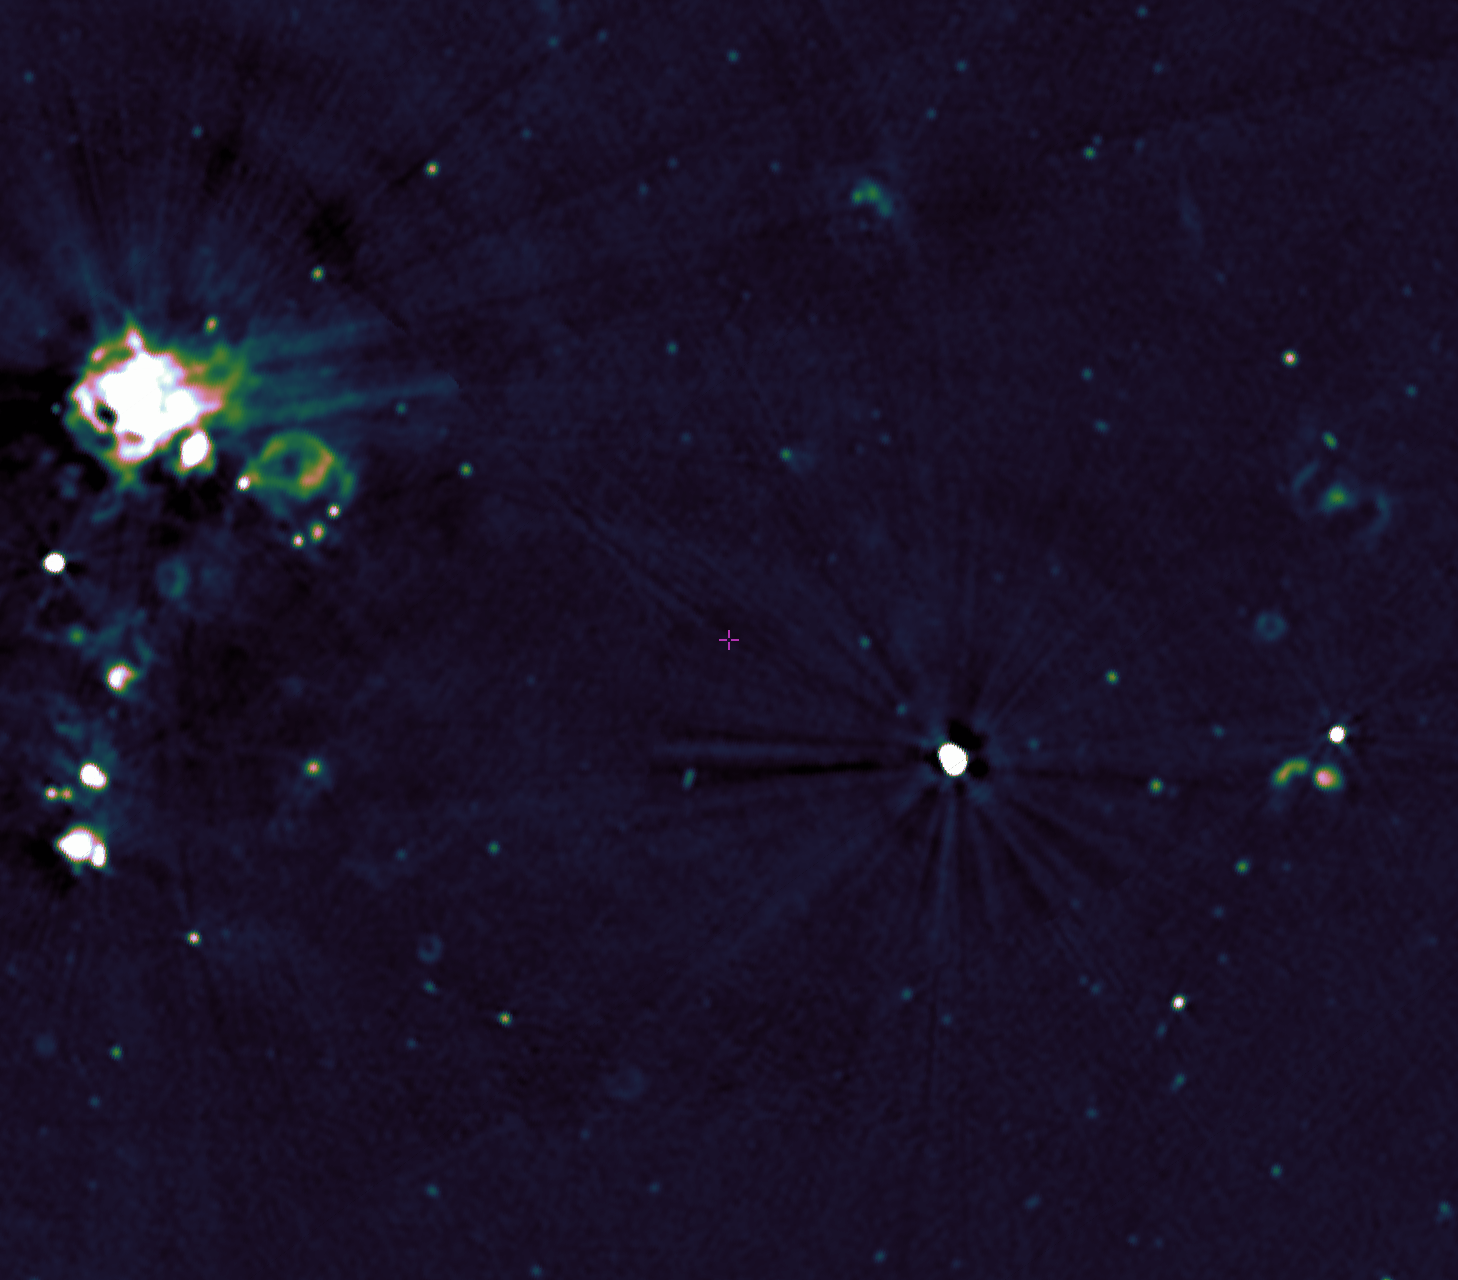
\includegraphics[width=1.0\linewidth]{./chapters/10.results/LMC/radio-843_cut.png}
		\caption{Radio wavelength at 843MHz.}
		\label{results:LMC:radio}
	\end{subfigure}
	\begin{subfigure}[b]{0.375\linewidth}
		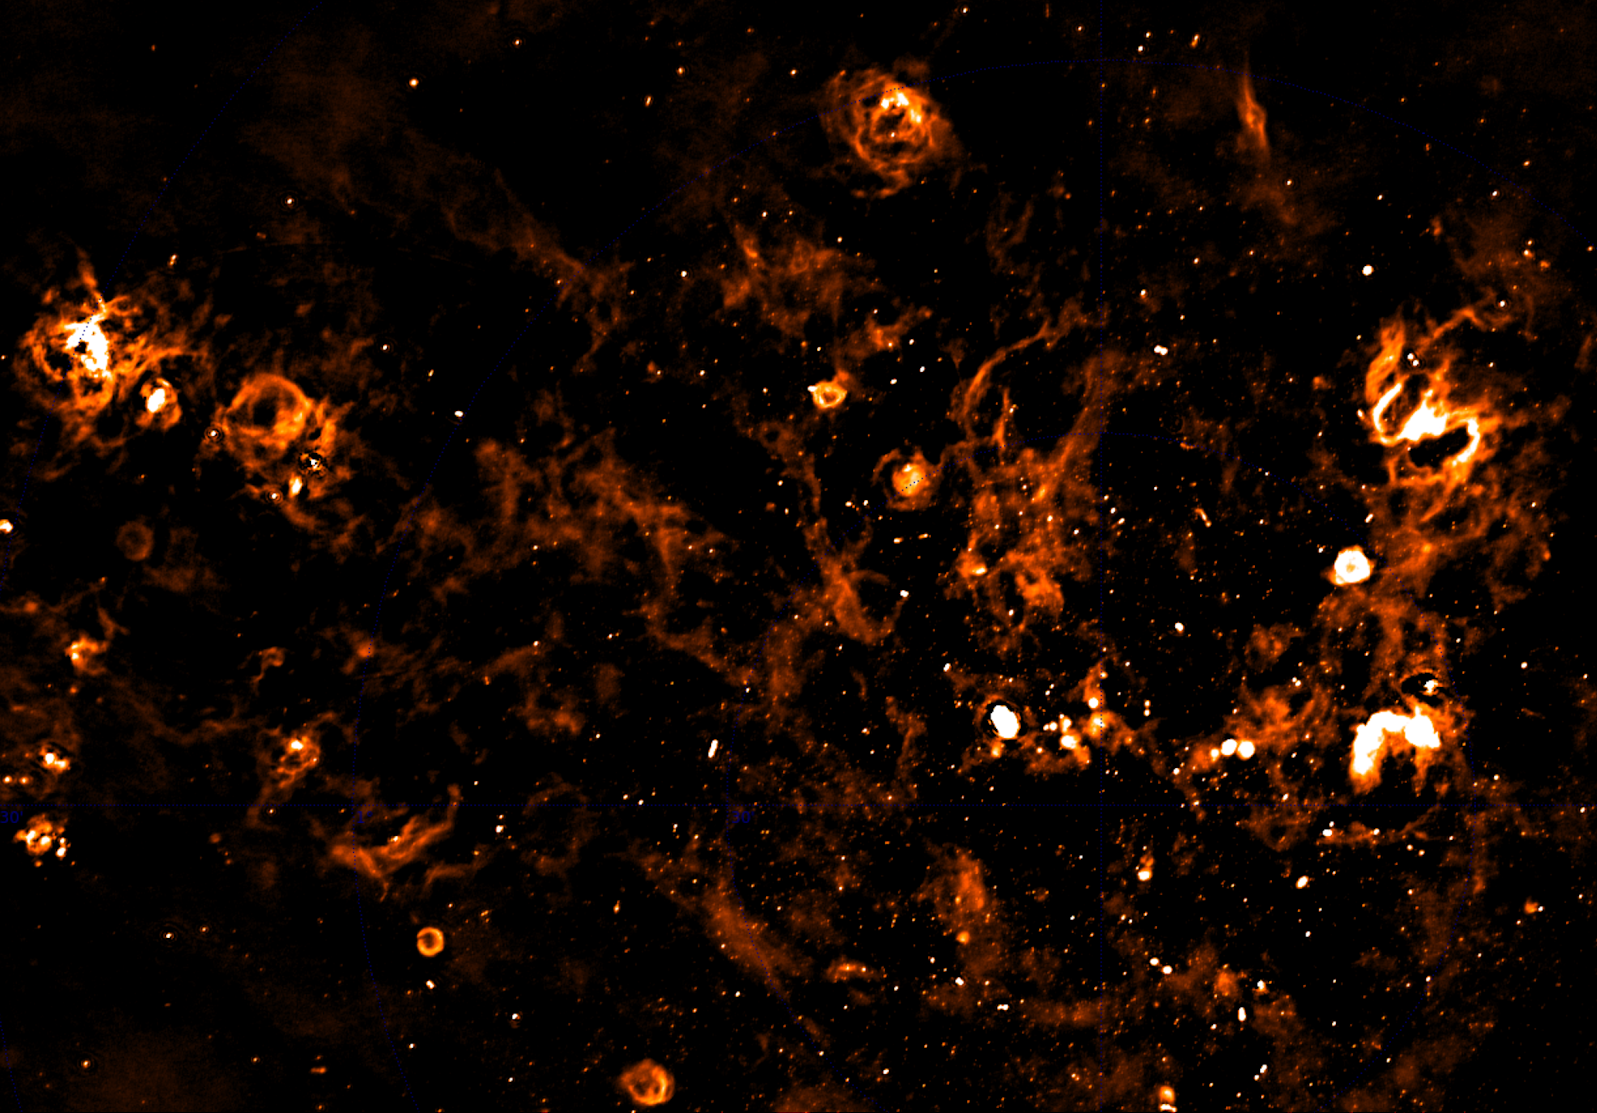
\includegraphics[width=1.0\linewidth]{./chapters/10.results/LMC/meerkat2.png}
		\caption{Wide band radio image by MeerKAT.}
		\label{results:LMC:meerkat}
	\end{subfigure}
	\caption{Section of the Large Magellanic Cloud (LMC)}
	\label{results:LMC}
\end{figure}

The MeerKAT observation covers a wide band of radio frequencies. The lowest frequency in the MeerKAT observation is 894 MHz, and the highest frequency is
Imaging the whole frequency band requires a wide band deconvolution algorithm. In wide band imaging, several images at different frequencies get deconvolved as an image cube. Wide band imaging again multiplies the amount of work that has to be done for reconstruction, as now we cannot deconvolve a single image, but have to deal with a whole image cube.

Wide band imaging is not possible within the time frame of this project. We take a narrow band subset of 5 channels from the original data (ranging from 1084 to 1088 MHz, about 1 Gb in size) for reconstruction. We also reduce the field-of-view to a more manageable section. Figure \ref{results:cutout} shows the LMC image section we are using together with a CLEAN reconstruction of the narrow band data.

\begin{figure}[h]
	\centering
	\begin{subfigure}[b]{0.4\linewidth}
		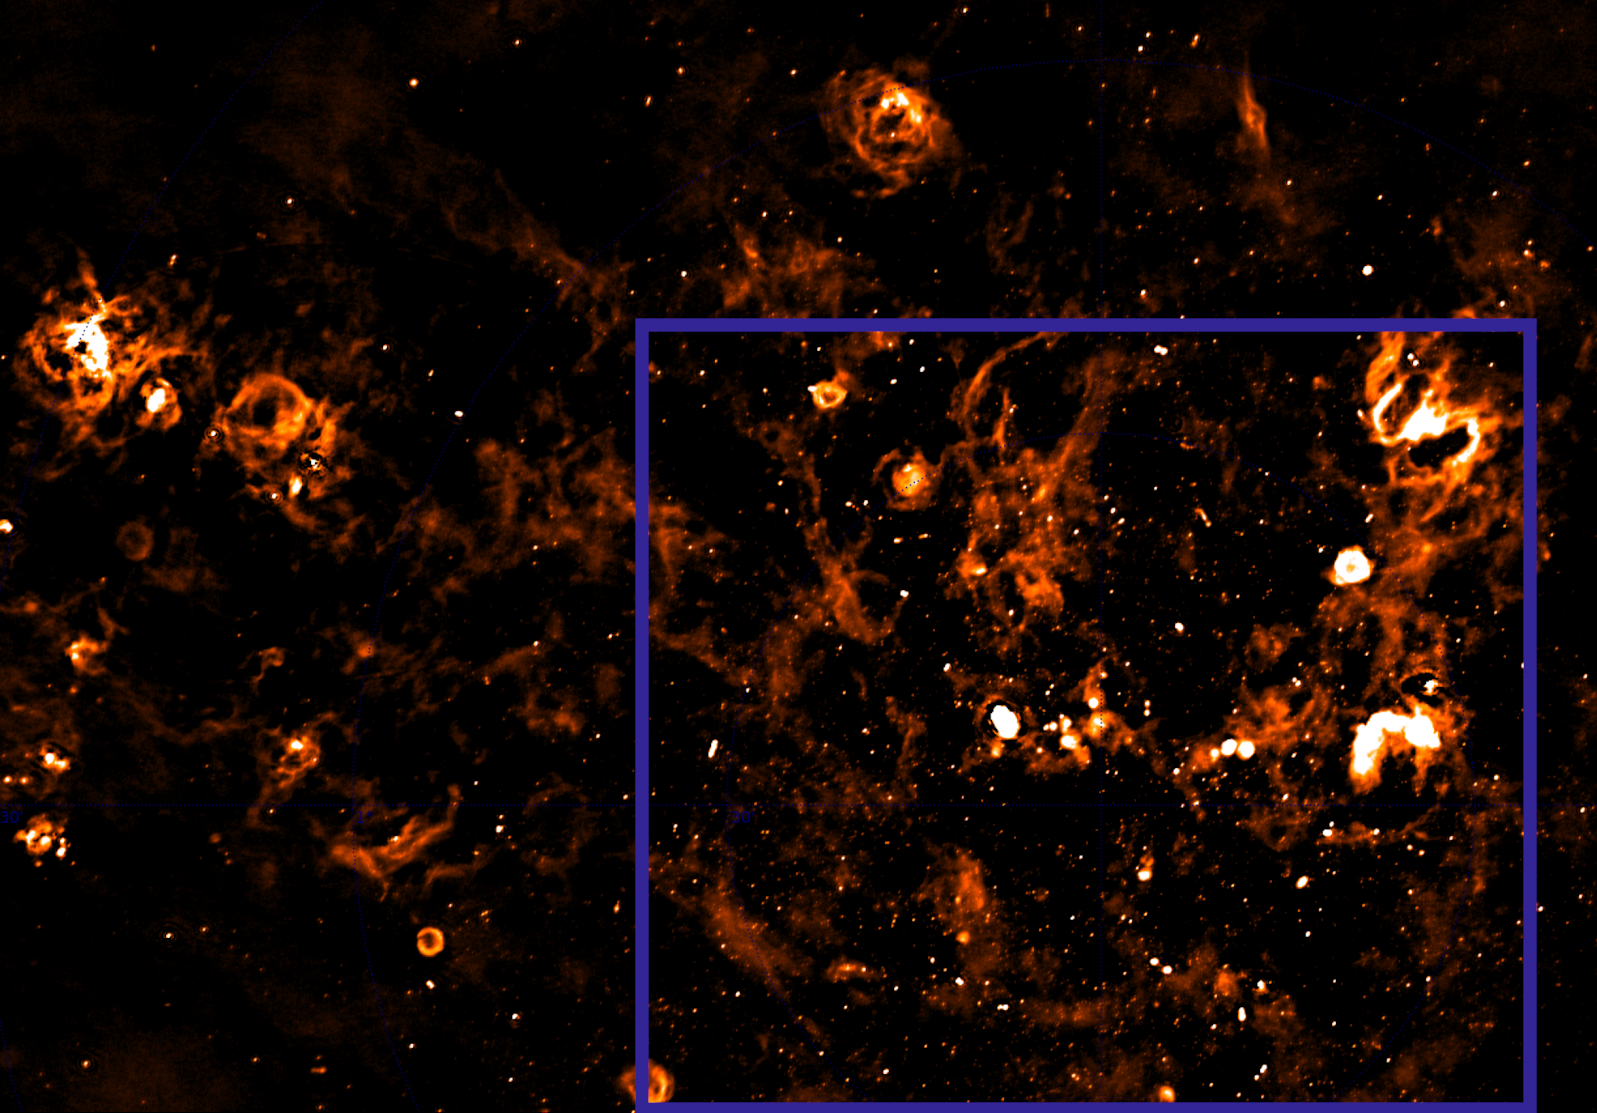
\includegraphics[width=1.0\linewidth]{./chapters/10.results/LMC/meerkat_cutout.png}
	\end{subfigure}
	\begin{subfigure}[b]{0.30\linewidth}
		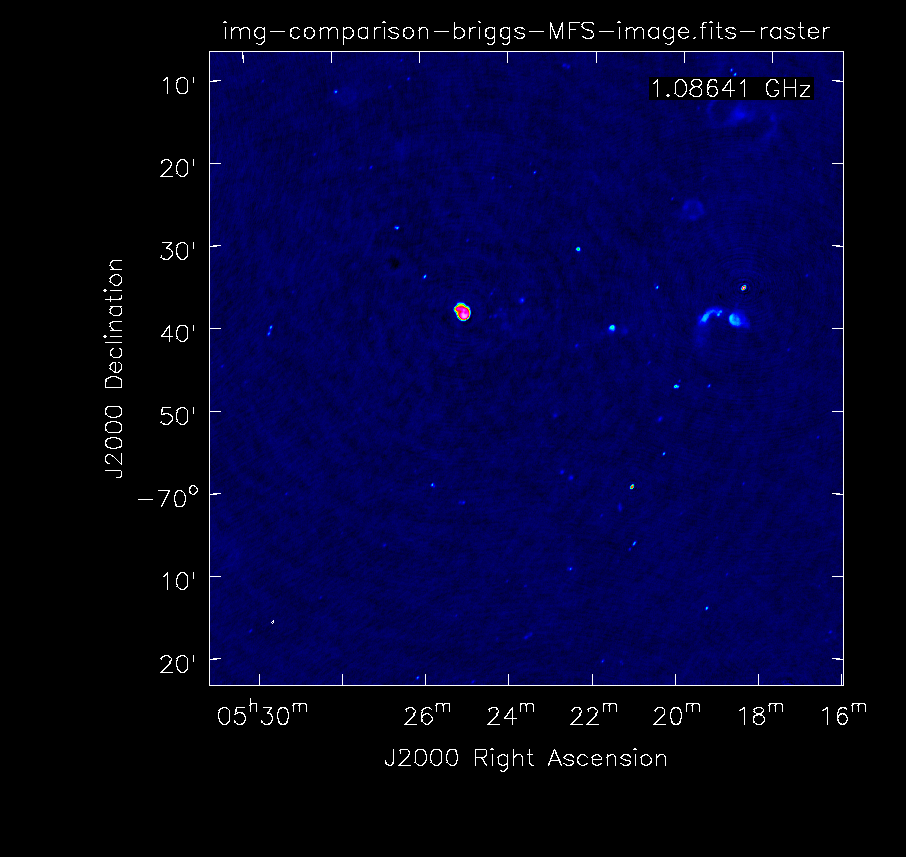
\includegraphics[width=1.0\linewidth]{./chapters/10.results/cleancomp/clean_briggs.png}
	\end{subfigure}
	\caption{Narrow band image section used.}
	\label{results:cutout}
\end{figure}

At the center of our image section \ref{results:cutout} we see the N132D supernova remnant. We partially see the faint extended emissions, although they are close to the noise level. This is known as a high-dynamic range reconstruction. We have strong radio sources mixed together with faint emissions, which are only marginally above the noise level of the image.

The total field-of-view of our image section is roughly 1.3 degrees(or 4600 arc seconds). Our reconstruction has $3072^2$ pixel with a resolution of 1.5 arc seconds per pixel. this is still a wide field-of-view reconstruction problem. We have to account for the effects of the $w$-term to achieve a high-dynamic range reconstruction.

In our test reconstruction, we need to account for $w$-term correction and high-dynamic range. We have excluded wide-band imaging as not feasible within the time frame of this project. In Section \ref{results:cleancomp} we compare the reconstructions of CLEAN with our coordinate descent based algorithm on the LMC observation. The next Section \ref{results:speedup} presents the speedup we achieve with coordinate descent by using our distributed or GPU-accelerated implementations.

In Section \ref{results:gradients} we show the core result of this project. Namely what effect has an approximate $PSF$ on the deconvolution problem and whether we can use it to further distribute the problem. The answer to that question is affirmative: We can approximate the $PSF$, and we can exploit it to further distribute the deconvolution. But we need more sophisticated coordinate descent algorithms to fully benefit from it.


\subsection{Comparison with CLEAN reconstructions} \label{results:cleancomp}
We use the WSCLEAN \cite{offringa2014wsclean} implementation of multi-scale CLEAN. We compare our coordinate descent reconstruction with two CLEAN reconstructions, oe with naturally weighted visibilities and one with briggs weighted visibilities.

There are three main visibility weighting scheme for the gridder that lead to different $PSF$s from the same measurements: Natural, uniform, and Briggs\cite{briggsWeighting}. Natural weighting scheme leads to an image with a lower noise level, but a wider $PSF$. Uniform weighting leads to a higher noise level, but to a $PSF$ whgich is more concentrated around a single pixel. Briggs weighting is a scheme combines the best from both worlds, receiving an image with acceptable noise level while getting a more concentrated $PSF$. As such it is widely used in radio astronomy image reconstruction. Our gridder implements the natural weighting scheme only. Nevertheless our coordinate descent algorithm is able to retrieve structures similar to the briggs-weighted multi-scale CLEAN reconstruction, even though coordinate descent has to work with a wider $PSF$.

\begin{figure}[h]
	\centering
	\begin{subfigure}[b]{0.4\linewidth}
		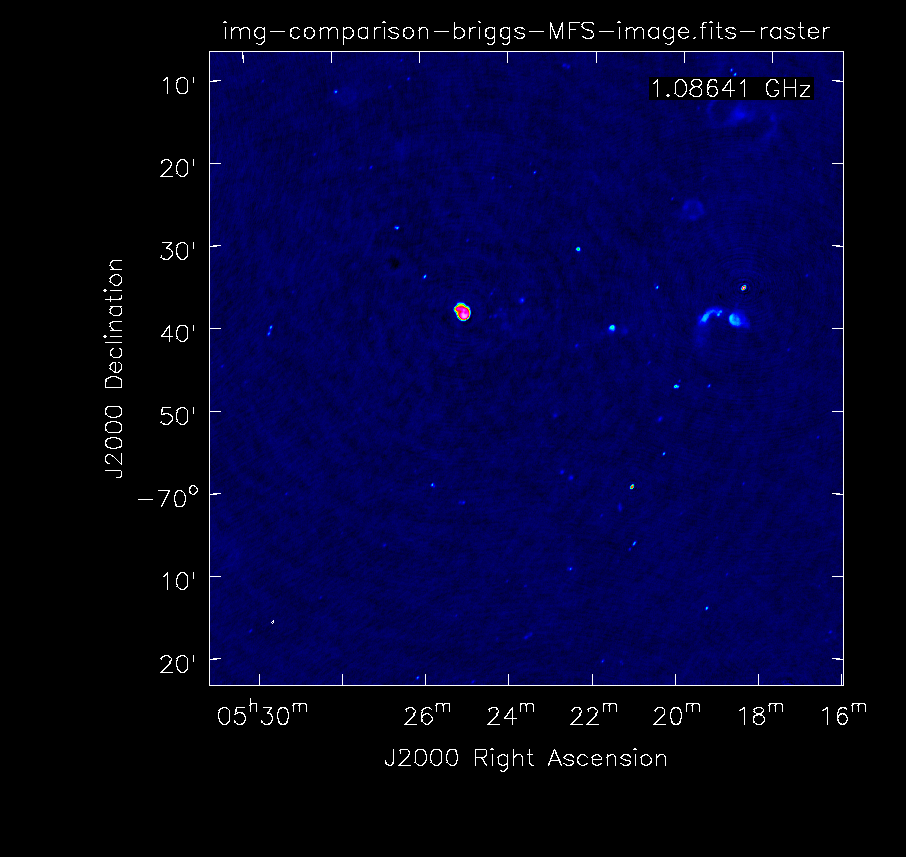
\includegraphics[width=1.00\linewidth]{./chapters/10.results/cleancomp/clean_briggs.png}
		\caption{Briggs weighted multi-scale CLEAN.}
		\label{results:comp:clean}
	\end{subfigure}
	\begin{subfigure}[b]{0.40\linewidth}
		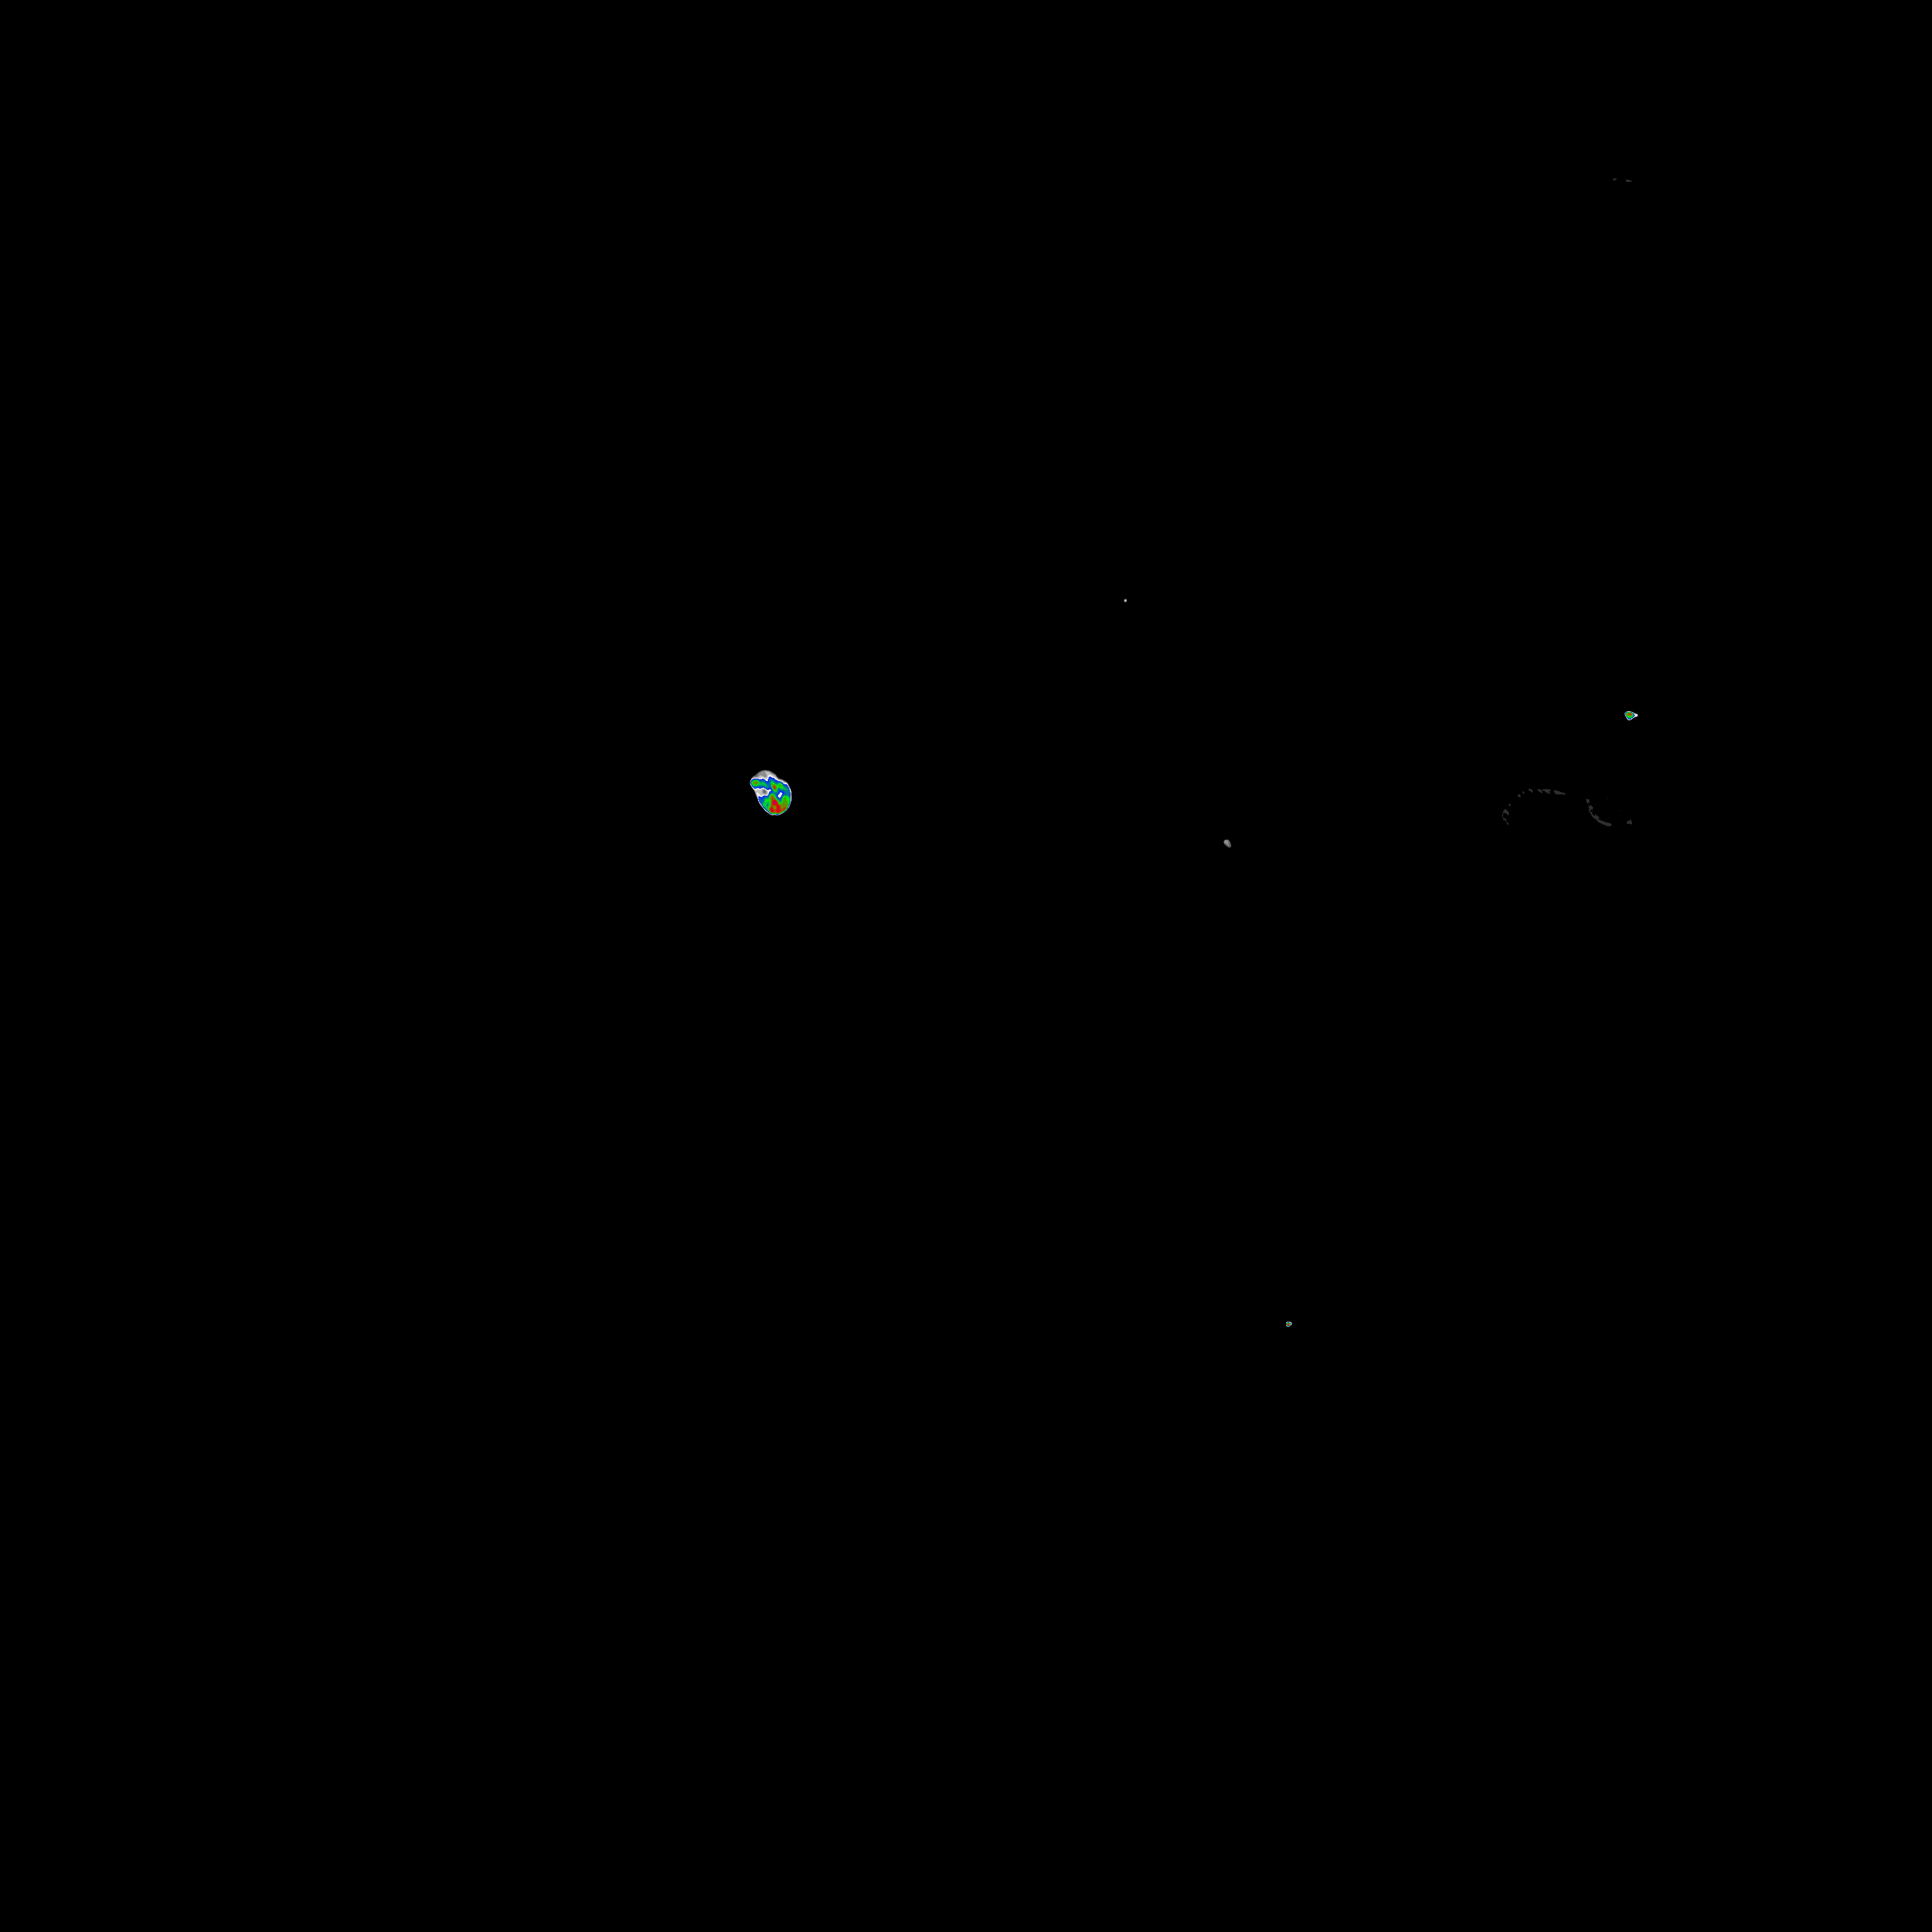
\includegraphics[width=1.00\linewidth]{./chapters/10.results/cleancomp/cd.png}
		\caption{Naturally weighted coordinate descent.}
		\label{results:comp:cd}
	\end{subfigure}
	\caption{Comparison of the whole image}
	\label{results:cleancomp:figure}
\end{figure}

Figure \ref{results:cleancomp:figure} shows the reconstruction of both briggs-weighted multi-scale CLEAN and the naturally weighted coordinate descent reconstruction.
%parameters for CLEAN and Coordinate descent. Lambda and alpha
CLEAN used 6 major cycles and 14 thousand minor cycle iterations. Our coordinate descent implementation converged after 5 major cycles and needed 100 thousand iterations to converge.

Coordinate descent needs a large number of iterations to converge when compared to multi-scale CLEAN. Note that a coordinate descent iteration is cheaper to compute than one iteration of multi-scale CLEAN. Also note that because we are searching for structures close to the noise level of the image, coordinate descent often adds pixels belonging to the noise in one major cycle, just to remove them in the next one. Path regularization\cite{friedman2010regularization} can combat this problem, and gets further investigated in the following Section \ref{results:gradients}.

Both algorithms detect the three extended emissions at the right side of the image. They detect various point sources at the same location. Coordinate descent and multi-scale CLEAN arrive at a roughly similar result. Coordinate descent detects similar structures in the N132 supernova remnant, as the briggs-weighted CLEAN, but also includes calibration errors in its reconstruction of the faint extended emissions.

\begin{figure}[h]
	\centering
	\begin{subfigure}[b]{0.3\linewidth}
		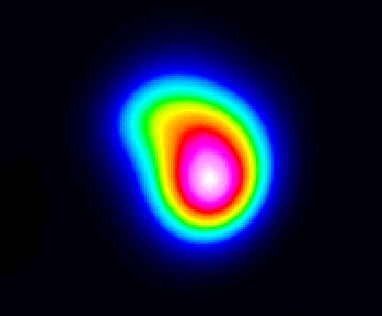
\includegraphics[width=1.00\linewidth]{./chapters/10.results/cleancomp/n132_clean.png}
		\caption{CLEAN Natural weighting.}
		\label{results:N132:clean}
	\end{subfigure}
	\begin{subfigure}[b]{0.3\linewidth}
		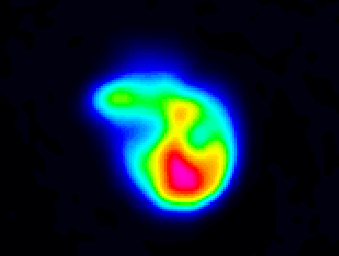
\includegraphics[width=1.00\linewidth]{./chapters/10.results/cleancomp/n132_clean_briggs.png}
		\caption{CLEAN Briggs weighting.}
		\label{results:N132:cleanbriggs}
	\end{subfigure}
	\begin{subfigure}[b]{0.3\linewidth}
		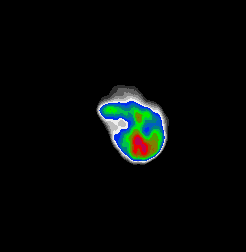
\includegraphics[width=1.00\linewidth]{./chapters/10.results/cleancomp/n132_cd.png}
		\caption{CD Natural weighting.}
		\label{results:comp:N132:cd}
	\end{subfigure}
	\caption{N132 comparison}
	\label{results:cleancomp::N132:figure}
\end{figure}

Figure \ref{results:cleancomp::N132:figure} compares the naturally-weighted CLEAN, briggs CLEAN and coordinate descent on the N132 supernova remnant. The naturally-weigted CLEAN and coordinate descent use the same $PSF$ for the deconvolution. But coordinate descent finds structures in N132 similar to the briggs-weighted CLEAN. Coordinate descent arrived at a plausible higher-resolved reconstruction of N132.

\begin{figure}[h]
	\centering
	\begin{subfigure}[b]{0.3\linewidth}
		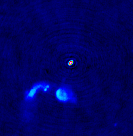
\includegraphics[width=1.00\linewidth]{./chapters/10.results/cleancomp/clean_calibration.png}
		\caption{Briggs CLEAN}
	\end{subfigure}
	\begin{subfigure}[b]{0.3\linewidth}
		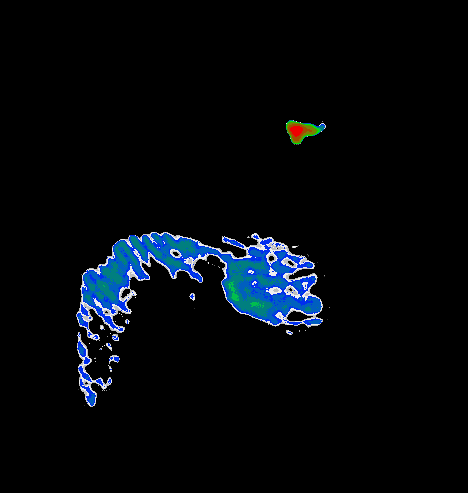
\includegraphics[width=1.00\linewidth]{./chapters/10.results/cleancomp/cd_calibration.png}
		\caption{Coordinate Descent}
	\end{subfigure}
	\caption{Influence of calibration errors}
	\label{results:cleancomp::calib:figure}
\end{figure}

Calibration errors on the other hand negatively influence the coordinate descent reconstruction. Figure \ref{results:cleancomp::calib:figure} shows a cutout of the right hand section of the reconstruction, where a faint extended emission is next to a point source with calibration errors. Multi-scale CLEAN is able to differentiate between the "ripples" from the calibration error, and the signal from the extended emission. Coordinate descent with the elastic net regularization includes the ripples into the reconstructed image. 

The only way to exclude the ripples from the reconstruction is to increase the regularization parameter $\lambda$., such as no pixel gets included which is not above the noise level + calibration error in the image. However, that would lead to other sources being "regularized away" in other regions of the image, which do not have a severe calibration error close by. 


\subsection{Coordinate descent acceleration with MPI or GPU}\label{results:speedup}
Describe hardware

Distributed with MPI

GPU implementation

Measurement of the speedup.

\begin{figure}[h]
	\centering
		\begin{subfigure}[b]{0.4\linewidth}
		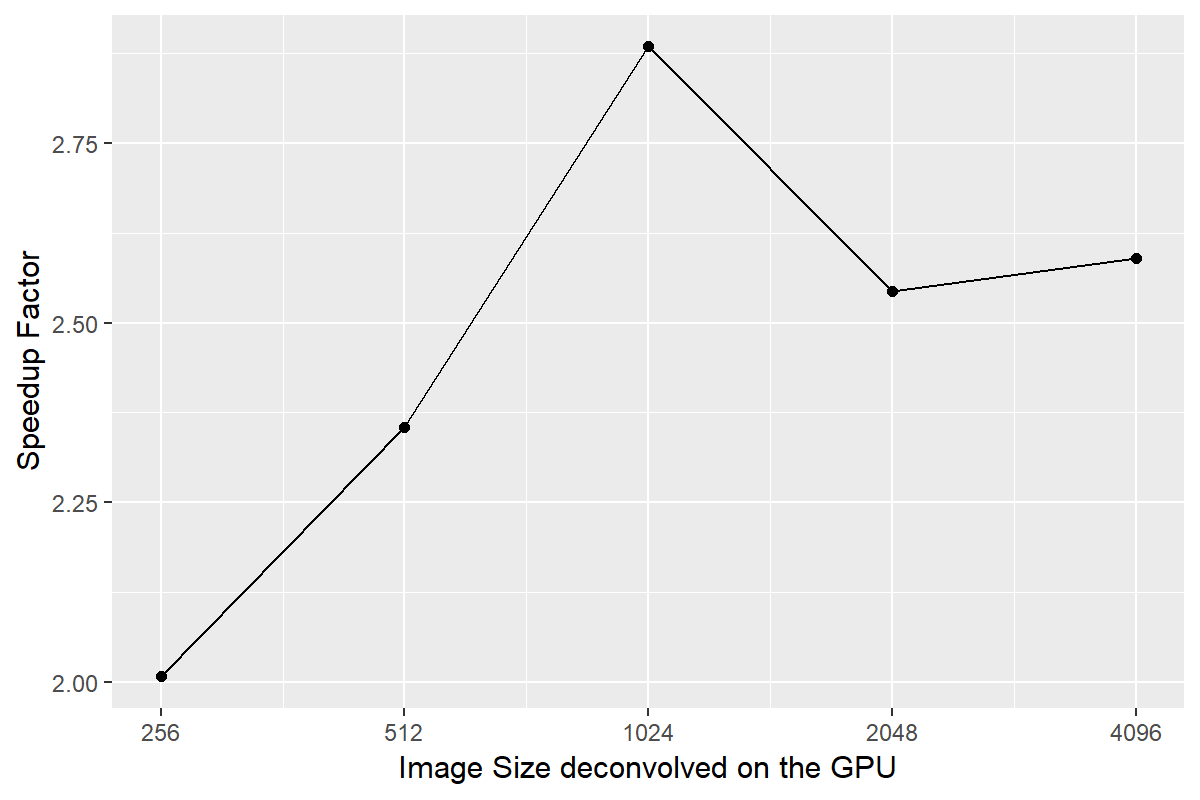
\includegraphics[width=1.00\linewidth]{./chapters/10.results/speedup/gpu.png}
	\end{subfigure}
	\begin{subfigure}[b]{0.4\linewidth}
		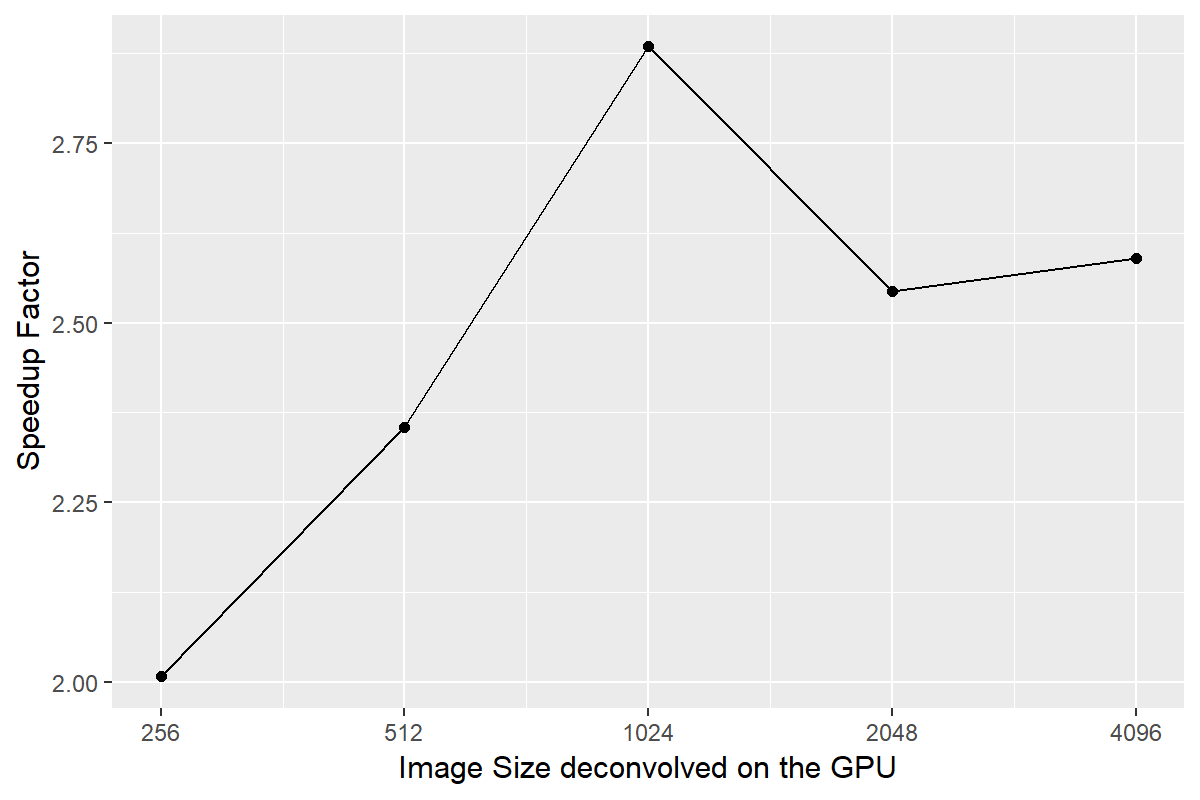
\includegraphics[width=1.00\linewidth]{./chapters/10.results/speedup/gpu.png}
	\end{subfigure}
	\caption{Speedup by using MPI or GPU acceleration}
	\label{results:speedup:figure}
\end{figure}


We cannot use MPI combined with the GPU. The MPI implementation uses a communication step in each coordinate descent iteration (communicating which pixel to optimize with MPI Allreduce). 



\subsection{Effect of approximating the $PSF$} \label{results:gradients}
As we described in Section \ref{gradients}, the $PSF$ for deconvolution is as big as the image. For wide field-of-view observations of MeerKAT, the $PSF$ is approximately a gaussian with decreasing pixel values the further we move from the center. Most of the values in the $PSF$ are close to zero. The question is, what effect has an approximate deconvolution with a smaller $PSF$? If we can approximate the deconvolution with a small enough $PSF$, we can solve patches of the image independently of each other. However, the $PSF$ approximation may need more major cycles to converge.

The effect of approximating the $PSF$ are not clear. We know that thanks to the $w$-term in the visibilities, the $PSF$ is not constant over the image. We already need several major cycles to converge. With a good approximation of the $PSF$, we may speed up the individual iterations of coordinate descent without needing more major cycle.

We presented two methods to approximating the $PSF$ for the deconvolution in Section \ref{gradients}. Method 1 updates only a fraction of the gradients, and Method 2 uses a fraction of the $PSF$ for deconvolution. We test both methods on the LMC data and explore what effects the approximations have on the reconstruction.

\subsubsection{Method 1: Approximate gradient update}
Our coordinate descent method updates the map of gradients after each iteration.  Method 1 starts with the same map of gradients as the original, but then only updates a fraction of the gradients in each iteration. It updates a rectangle of the most significant gradients.With each coordinate descent iteration, the map of gradients gets less accurate. Because we do an approximate update of gradients, this method should converge to the same result as the original with enough major cycles.

At the beginning of each major cycle, we calculate the objective value of the current solution. We compare the objective value and the wall-clock time of the original and the approximate gradient update. This is a minimization problem, meaning the lowest objective is the most accurate reconstruction (according to the elastic net regularization).

\begin{figure}[h]
	\centering
	\begin{subfigure}[b]{0.7\linewidth}
		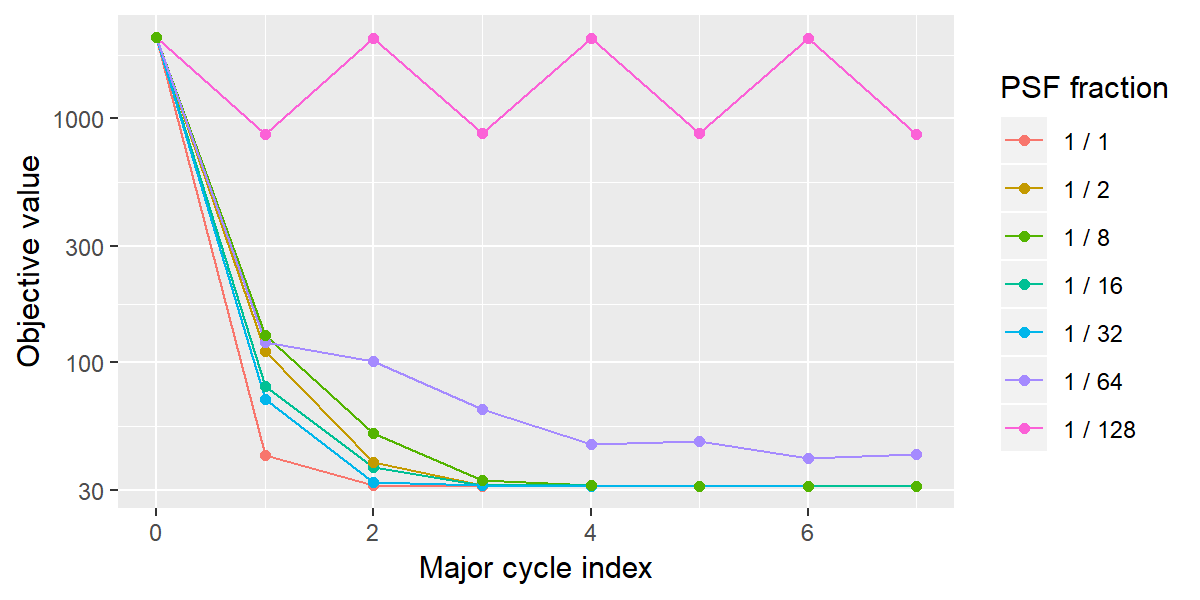
\includegraphics[width=\linewidth]{./chapters/10.results/gradient/ApproxUpdate/size.png}
	\end{subfigure}
	\\
	\begin{subfigure}[b]{0.35\linewidth}
		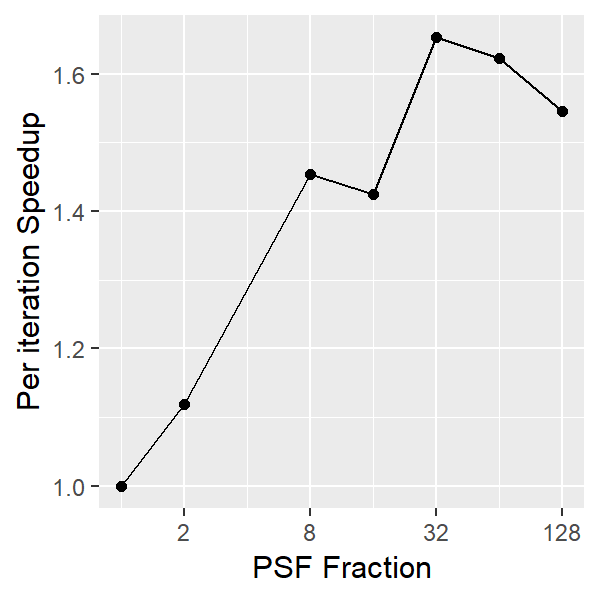
\includegraphics[width=\linewidth]{./chapters/10.results/gradient/ApproxUpdate/speedup_iter.png}
	\end{subfigure}
	\begin{subfigure}[b]{0.35\linewidth}
		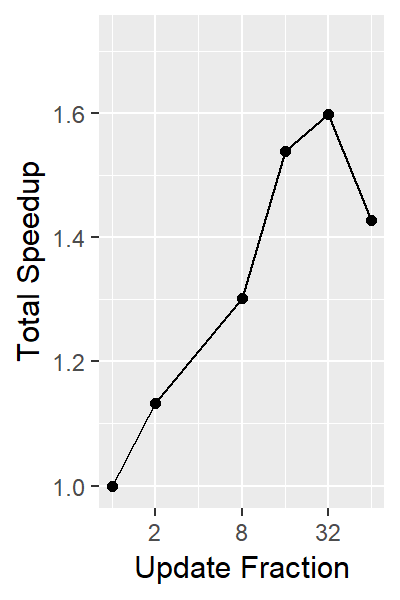
\includegraphics[width=\linewidth]{./chapters/10.results/gradient/ApproxUpdate/speedup_total.png}
	\end{subfigure}
	
	\caption{Effect of only updating a fraction of the gradients.}
	\label{results:gradients:update}
\end{figure}

The smallest fraction of gradient updater, for which coordinate still converges is $\frac{1}{64}$ of the total update. Meaning, we can update only a rectangle of $48^2$ pixels, or an image patch of 72 arc-seconds in size. However, it is obvious from the Figure \ref{results:gradients:update} that coordinate descent needs more major cycles to converge with such an extreme approximation.

With less extreme approximations, we also reduce the number of necessary major cycles. The approximation of $\frac{1}{32}$ needs two more major cycle, while all other need the one more as the original method\footnote{6 cycles to converge, and one extra cycle which is here to measure the final objective}. The objective values of the approximations end within 0.03\% of the original(the objective value of the approximations are higher by a factor of 0.0003).

Figure \ref{results:gradients:update} also shows two speedup comparisons. The speedup from the approximation is harder to quantify. For one, each iteration of coordinate descent becomes cheaper, because we only update a small part of the gradient map. This is the per iteration speedup. The second speedup Figure compares the overall time spent in deconvolution. Although each iteration becomes cheaper with the approximation, we may need more iterations to converge. Also, we have an implicit path regularization in the approximation. Therefore, a speedup per coordinate descent iteration does not necessarily lead to an overall speedup.

As we discussed in section In Section \ref{gradients:pathreg}, we have a limit in each major cycle to how far we can trust our approximation. That is why in the first major cycle coordinate descent gets started with a higher $\lambda$ regularization than specified. In each successive major cycle, we reduce the $\lambda$ parameter until we reach the specified value. This is an implicit form of path regularization, and may help speeding up the convergence rate of coordinate descent in general \cite{friedman2010regularization}. In our case, we need path regularization to ensure convergence over several major cycles (Aggressive approximations like $\frac{1}{64}$ start to oscillate over several major cycle). Notice that the overall speedup in Figure \ref{results:gradients:update} is lower than the speedup we get per iteration. This suggests path regularization as implemented here does not speed up convergence rate.

Overall with gradient update approximations give us a speedup factor of around 1.5. Depending on how aggressive we approximate, We need one or two more major cycles than the original coordinate descent deconvolutions. This puts gradient update approximations on par with multi-scale CLEAN in terms of major cycles. 

\subsubsection{Method 2: Approximate deconvolution}
In this method, we use a fraction of the total $PSF$ for deconvolution. This method solves a different deconvolution problem, where the $PSF$ is for example only $\frac{1}{8}$ the size. The downside is that method 2 is not guaranteed to converge to the same optimum. Nevertheless, we solve the approximate deconvolution problem with several different fractions of the $PSF$ and compare how close the approximate solution is to the original.

As before, we measure the true objective value for the approximate solution at the beginning of each major cycle iteration. The Figure \ref{results:gradients:aproxDeconv} compares the approximate deconvolution to the original.

\begin{figure}[h]
	\centering
	\begin{subfigure}[b]{0.7\linewidth}
		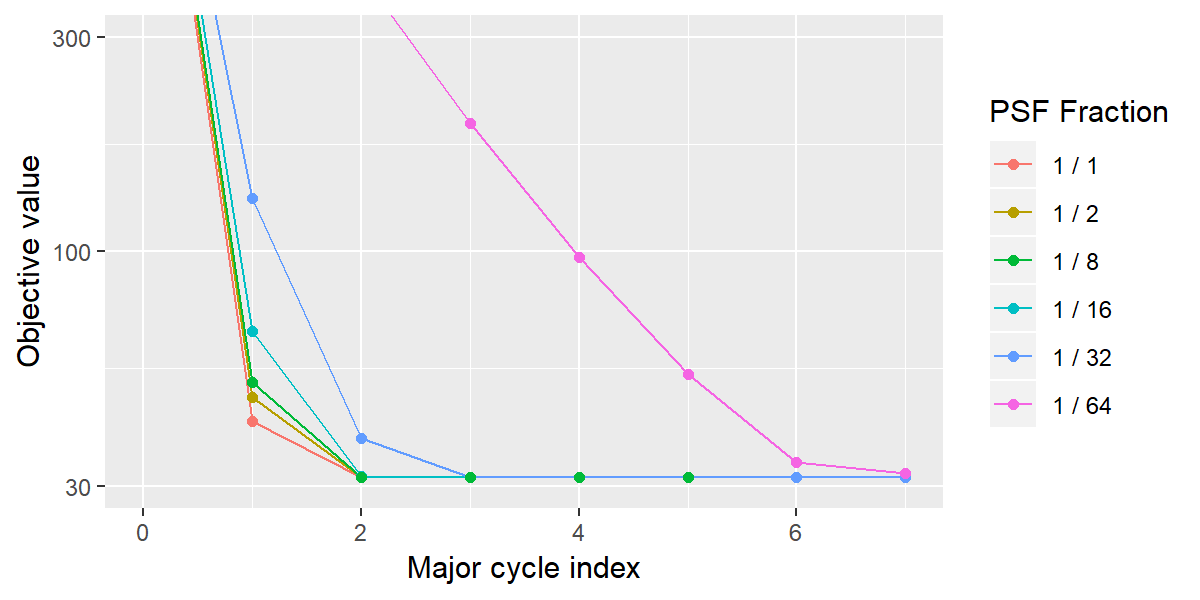
\includegraphics[width=\linewidth]{./chapters/10.results/gradient/ApproxDeconv/size.png}
	\end{subfigure}
	\\
	\begin{subfigure}[b]{0.35\linewidth}
		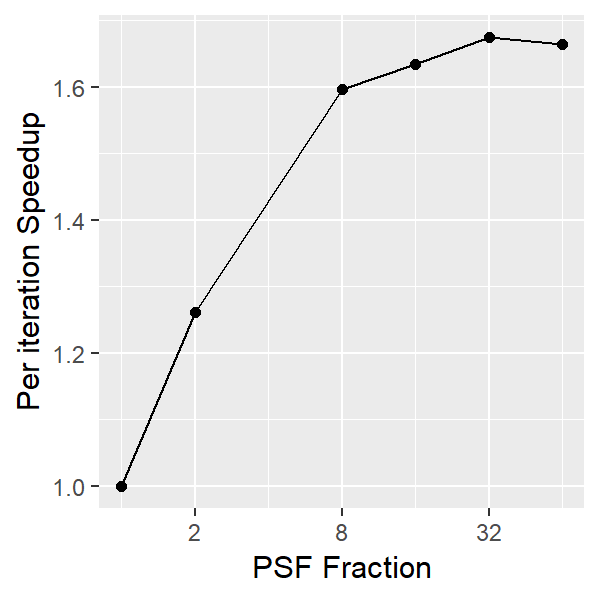
\includegraphics[width=\linewidth]{./chapters/10.results/gradient/ApproxDeconv/speedup_iter.png}
	\end{subfigure}
	\begin{subfigure}[b]{0.35\linewidth}
		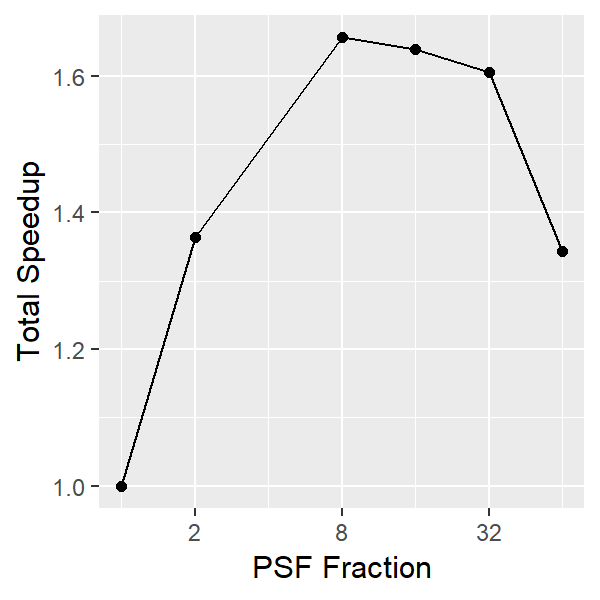
\includegraphics[width=\linewidth]{./chapters/10.results/gradient/ApproxDeconv/speedup_total.png}
	\end{subfigure}
	
	\caption{Effect of the L1 and L2 Norm separately.}
	\label{results:gradients:aproxDeconv}
\end{figure}

The performance is similar to the first method at first glance. Both methods converge in a similar manner, with a similar factor of speedup. For the $PSF$ fraction $\frac{1}{64}$ this is largely due to the same path regularization used in this method. For larger $PSF$'s, starting from $\frac{1}{16}$, the path regularization becomes less important with this method, as it only effects the regularization parameter $\lambda$ of major cycle index 0. Indeed, this method is less likely to oscillate and seems to have a more stable convergence.

The approximate deconvolution converges faster than the first method. At the start of the same major cycle, this method always has a lower objective. However, it is not guaranteed to converge to the same result. This can be seen in the fact that it never reaches the same objective value as the original. The objective value of the approximation is within 0.07\% (Factor of 0.0007, roughly twice the factor of the first method). The difference gets more significant, the more extreme we chose the deconvolution approximation.

Nevertheless, the approximate deconvolution converges surprisingly close to the original solution. The question is, is this difference of 0.07\% in the objective value significant? The answer to this question depends on what kind of error the approximation introduces in the image. The obvious error is that the approximation chronically under-estimates the pixel values: The maximum pixel value in N132 of the original is 0.0024 Jansky/beam, while the maximum of the $\frac{1}{16}$ approximation is 0.00235 Jansky/beam. The pixel magnitude is important in the self-calibration regime \cite{offringa2017optimized} (When we take the result of the reconstruction and try to improve the calibration).

The under-approximation of pixel values is an error we cannot ignore. One naive remedy is to start with the deconvolution approximation, but switch to the original $PSF$ after a certain number of major cycle. This would give us the guarantee to converge to the same result, but let us use an approximation at the start. We propose another solution: Combining the two approximation methods.


\subsubsection{Combination of Method 1 and 2}\label{results:gradients:comparison}
The two approximation methods have two different shortcomings: Approximate gradient update (method 1) converges more slowly, and converges to the same result as the original. Approximate deconvolution (method 2) converges faster than method 1, but does not converge to the same result. Here, we combine the two methods to remedy the shortcomings: For the first couple of major cycles, we use approximate deconvolution, and then switch to approximate gradient update.

We compare the original, approximate gradient update, approximate deconvolution and our combination in. We use the factor $\frac{1}{16}$ for approximations, meaning we update $\frac{1}{16}$ of the gradients, and do the approximate deconvolution with $\frac{1}{16}$ of the $PSF$.

\begin{figure}[h]
	\centering
	\begin{subfigure}[b]{0.33\linewidth}
		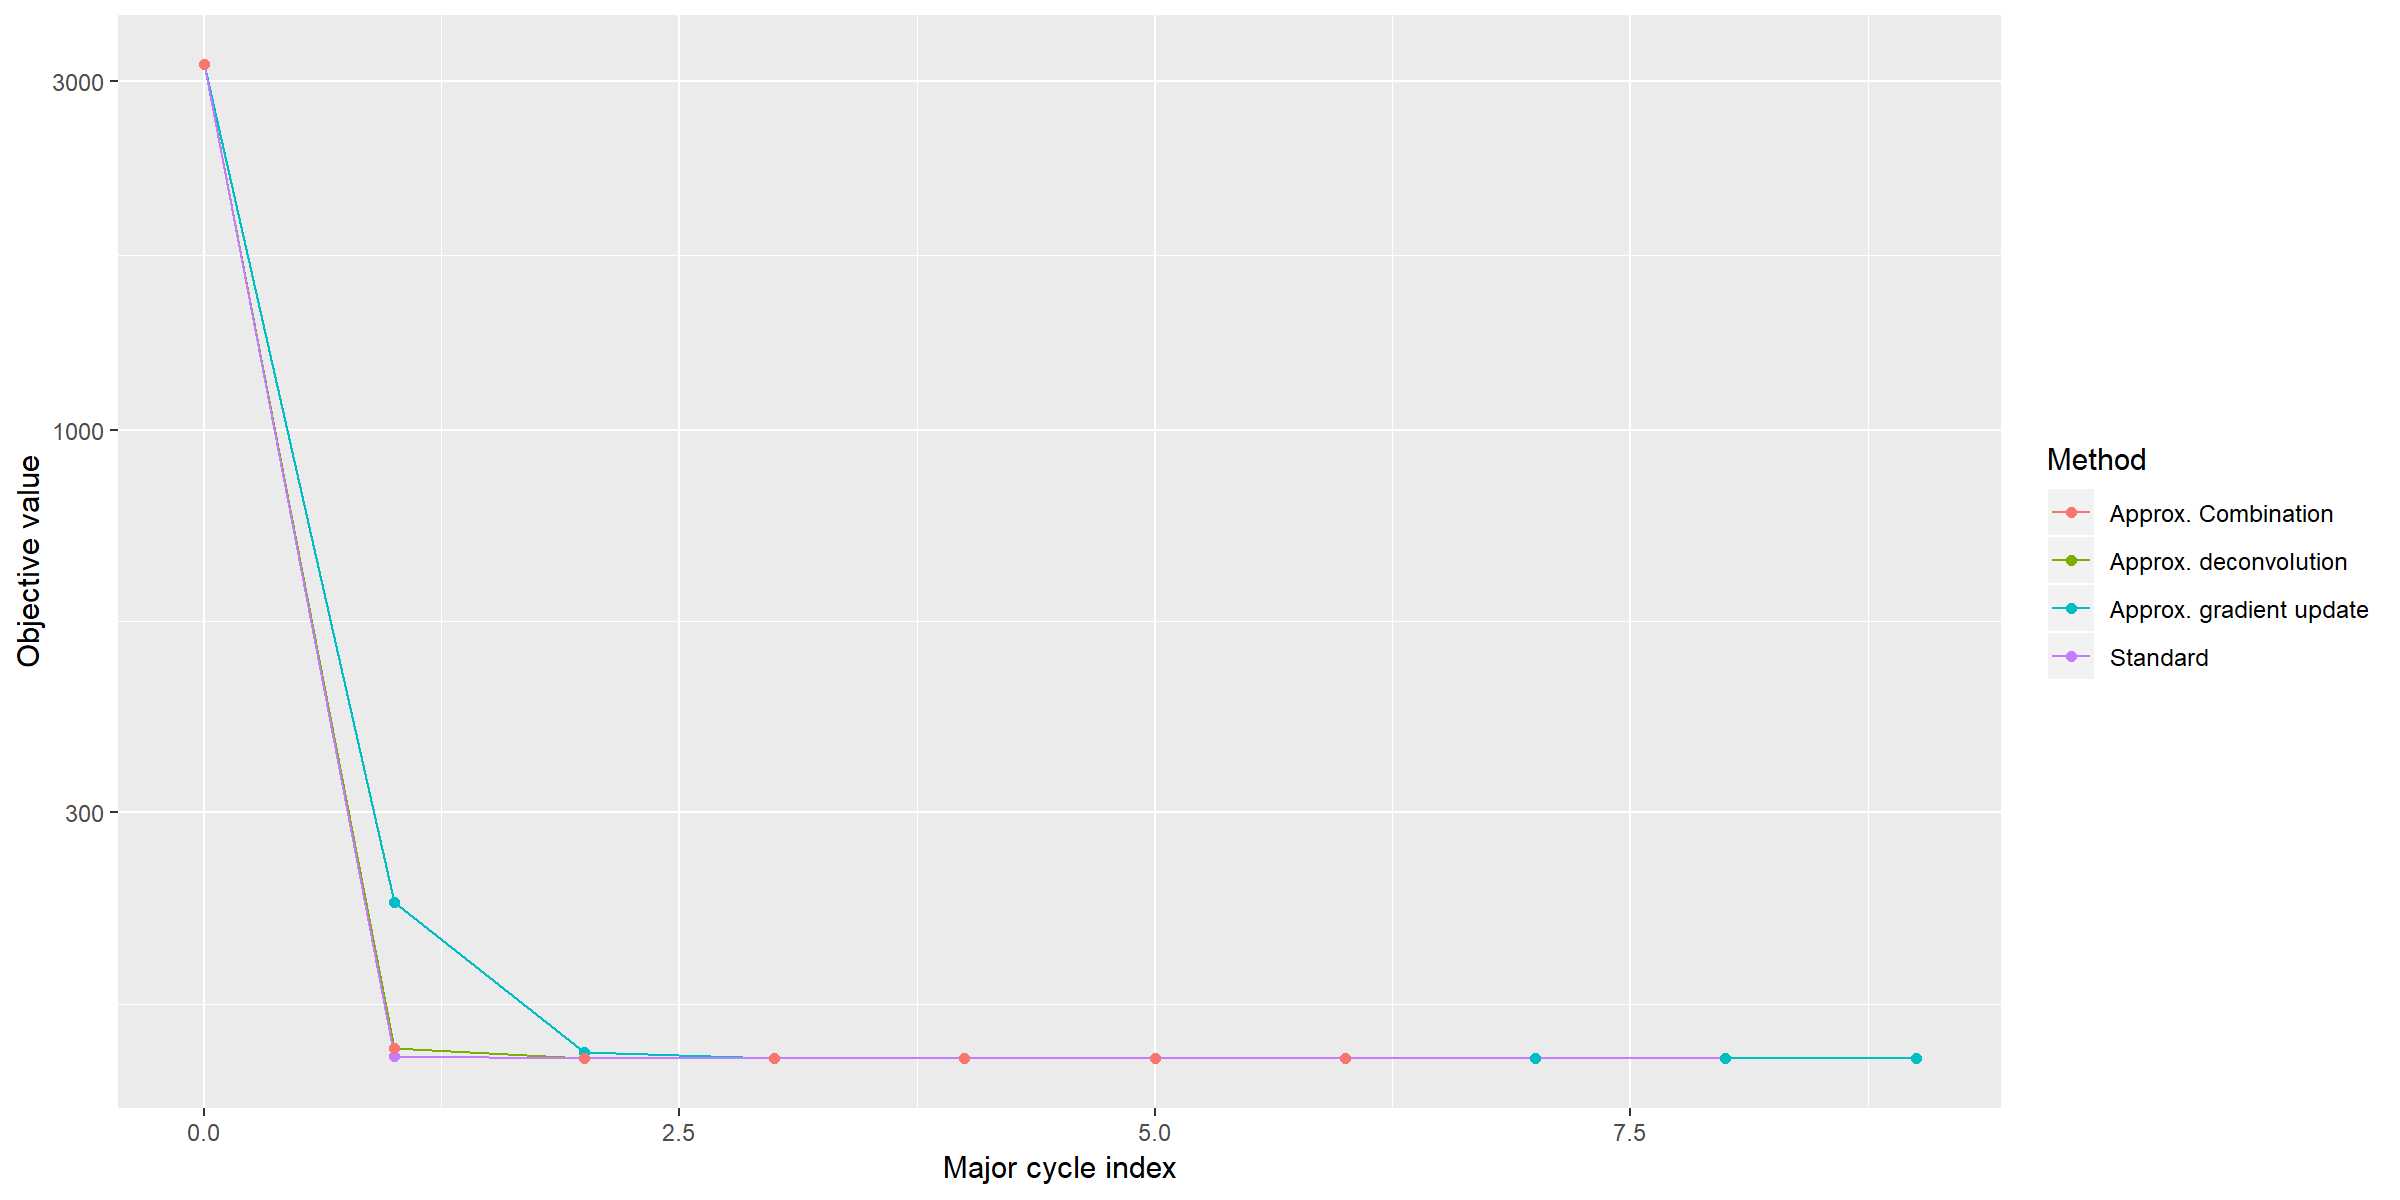
\includegraphics[width=\linewidth]{./chapters/10.results/gradient/comparison.png}
	\end{subfigure}
	\begin{subfigure}[b]{0.66\linewidth}
		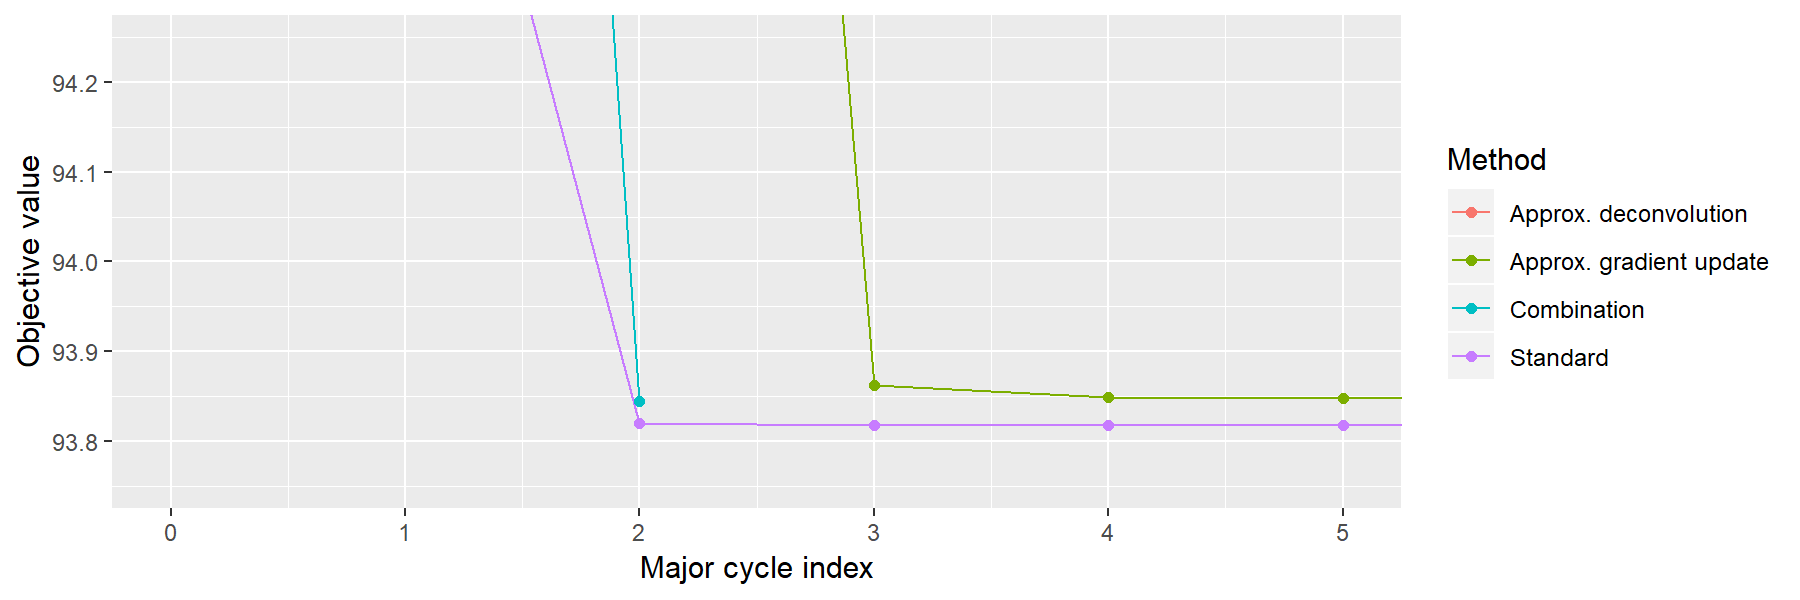
\includegraphics[width=\linewidth]{./chapters/10.results/gradient/comparison_zoom.png}
	\end{subfigure}
	
	\caption{Comparison of the two methods using the fraction $\frac{1}{16}$ of the $PSF$.}
	\label{results:gradients:comparison:figure}
\end{figure}

 Figure \ref{results:gradients:comparison:figure}

We switch from approximate deconvolution to gradient update after the path regularization has reached the target $\lambda$ for the first time. In the case of the LMC data, the implementation uses approximate deconvolution for major cycle index 0 and 1, and then switches to approximate gradient update.



Convergence. With the combination, we move actually below the original solution. 
Approximation errors are not correlated.

\begin{center}
	\begin{tabular}{ c||c|c } 
		\hline
		Method & Iteration Speedup & Total Speedup \\ \hline \hline
		Original & 1.00 & 1.00 \\ 
		(Method 1) Approx. gradient update & 1.66 & 1.55 \\ 
		(Method 2) Approx. deconvolution & 1.67 & 1.68 \\ \hline
		Combination & 1.69 & 1.68 \\ 
		\hline
	\end{tabular}
\label{results:gradients:comparison:speedup}
\end{center}
What about the speedup?

Show images

\subsubsection{Masking the $PSF$}
